% Created by tikzDevice version 0.12.6 on 2026-08-03 04:28:34
% !TEX encoding = UTF-8 Unicode
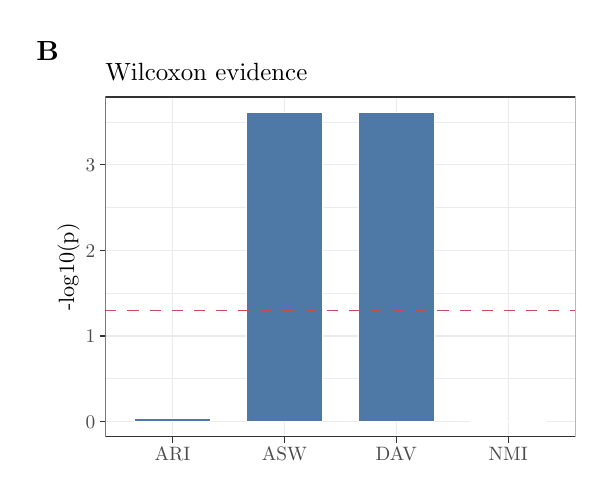
\begin{tikzpicture}[x=1pt,y=1pt]
\definecolor{fillColor}{RGB}{255,255,255}
\path[use as bounding box,fill=fillColor,fill opacity=0.00] (0,0) rectangle (201.01,161.83);
\begin{scope}
\path[clip] (  1.11,  1.74) rectangle (199.90,160.09);
\definecolor{drawColor}{RGB}{255,255,255}
\definecolor{fillColor}{RGB}{255,255,255}

\path[draw=drawColor,line width= 0.4pt,line join=round,line cap=round,fill=fillColor] (  1.11,  1.74) rectangle (199.90,160.09);
\end{scope}
\begin{scope}
\path[clip] ( 28.07, 13.93) rectangle (197.90,136.79);
\definecolor{fillColor}{RGB}{255,255,255}

\path[fill=fillColor] ( 28.07, 13.93) rectangle (197.90,136.79);
\definecolor{drawColor}{gray}{0.92}

\path[draw=drawColor,line width= 0.2pt,line join=round] ( 28.07, 34.98) --
	(197.90, 34.98);

\path[draw=drawColor,line width= 0.2pt,line join=round] ( 28.07, 65.89) --
	(197.90, 65.89);

\path[draw=drawColor,line width= 0.2pt,line join=round] ( 28.07, 96.81) --
	(197.90, 96.81);

\path[draw=drawColor,line width= 0.2pt,line join=round] ( 28.07,127.73) --
	(197.90,127.73);

\path[draw=drawColor,line width= 0.4pt,line join=round] ( 28.07, 19.52) --
	(197.90, 19.52);

\path[draw=drawColor,line width= 0.4pt,line join=round] ( 28.07, 50.43) --
	(197.90, 50.43);

\path[draw=drawColor,line width= 0.4pt,line join=round] ( 28.07, 81.35) --
	(197.90, 81.35);

\path[draw=drawColor,line width= 0.4pt,line join=round] ( 28.07,112.27) --
	(197.90,112.27);

\path[draw=drawColor,line width= 0.4pt,line join=round] ( 52.33, 13.93) --
	( 52.33,136.79);

\path[draw=drawColor,line width= 0.4pt,line join=round] ( 92.77, 13.93) --
	( 92.77,136.79);

\path[draw=drawColor,line width= 0.4pt,line join=round] (133.20, 13.93) --
	(133.20,136.79);

\path[draw=drawColor,line width= 0.4pt,line join=round] (173.64, 13.93) --
	(173.64,136.79);
\definecolor{drawColor}{RGB}{255,255,255}
\definecolor{fillColor}{RGB}{78,121,167}

\path[draw=drawColor,line width= 0.2pt,fill=fillColor] (159.89, 19.52) rectangle (187.39, 19.53);

\path[draw=drawColor,line width= 0.2pt,fill=fillColor] ( 38.58, 19.52) rectangle ( 66.08, 20.58);

\path[draw=drawColor,line width= 0.2pt,fill=fillColor] ( 79.02, 19.52) rectangle (106.52,131.21);

\path[draw=drawColor,line width= 0.2pt,fill=fillColor] (119.46, 19.52) rectangle (146.95,131.21);
\definecolor{drawColor}{RGB}{196,78,82}

\path[draw=drawColor,line width= 0.4pt,dash pattern=on 4pt off 4pt ,line join=round] ( 28.07, 59.74) -- (197.90, 59.74);
\definecolor{drawColor}{gray}{0.20}

\path[draw=drawColor,line width= 0.4pt,line join=round,line cap=round] ( 28.07, 13.93) rectangle (197.90,136.79);
\end{scope}
\begin{scope}
\path[clip] (  0.00,  0.00) rectangle (201.01,161.83);
\definecolor{drawColor}{gray}{0.30}

\node[text=drawColor,anchor=base east,inner sep=0pt, outer sep=0pt, scale=  0.70] at ( 24.47, 17.11) {0};

\node[text=drawColor,anchor=base east,inner sep=0pt, outer sep=0pt, scale=  0.70] at ( 24.47, 48.02) {1};

\node[text=drawColor,anchor=base east,inner sep=0pt, outer sep=0pt, scale=  0.70] at ( 24.47, 78.94) {2};

\node[text=drawColor,anchor=base east,inner sep=0pt, outer sep=0pt, scale=  0.70] at ( 24.47,109.86) {3};
\end{scope}
\begin{scope}
\path[clip] (  0.00,  0.00) rectangle (201.01,161.83);
\definecolor{drawColor}{gray}{0.20}

\path[draw=drawColor,line width= 0.4pt,line join=round] ( 26.07, 19.52) --
	( 28.07, 19.52);

\path[draw=drawColor,line width= 0.4pt,line join=round] ( 26.07, 50.43) --
	( 28.07, 50.43);

\path[draw=drawColor,line width= 0.4pt,line join=round] ( 26.07, 81.35) --
	( 28.07, 81.35);

\path[draw=drawColor,line width= 0.4pt,line join=round] ( 26.07,112.27) --
	( 28.07,112.27);
\end{scope}
\begin{scope}
\path[clip] (  0.00,  0.00) rectangle (201.01,161.83);
\definecolor{drawColor}{gray}{0.20}

\path[draw=drawColor,line width= 0.4pt,line join=round] ( 52.33, 11.93) --
	( 52.33, 13.93);

\path[draw=drawColor,line width= 0.4pt,line join=round] ( 92.77, 11.93) --
	( 92.77, 13.93);

\path[draw=drawColor,line width= 0.4pt,line join=round] (133.20, 11.93) --
	(133.20, 13.93);

\path[draw=drawColor,line width= 0.4pt,line join=round] (173.64, 11.93) --
	(173.64, 13.93);
\end{scope}
\begin{scope}
\path[clip] (  0.00,  0.00) rectangle (201.01,161.83);
\definecolor{drawColor}{gray}{0.30}

\node[text=drawColor,anchor=base,inner sep=0pt, outer sep=0pt, scale=  0.70] at ( 52.33,  5.51) {ARI};

\node[text=drawColor,anchor=base,inner sep=0pt, outer sep=0pt, scale=  0.70] at ( 92.77,  5.51) {ASW};

\node[text=drawColor,anchor=base,inner sep=0pt, outer sep=0pt, scale=  0.70] at (133.20,  5.51) {DAV};

\node[text=drawColor,anchor=base,inner sep=0pt, outer sep=0pt, scale=  0.70] at (173.64,  5.51) {NMI};
\end{scope}
\begin{scope}
\path[clip] (  0.00,  0.00) rectangle (201.01,161.83);
\definecolor{drawColor}{RGB}{0,0,0}

\node[text=drawColor,rotate= 90.00,anchor=base,inner sep=0pt, outer sep=0pt, scale=  0.80] at ( 16.80, 75.36) {-log10(p)};
\end{scope}
\begin{scope}
\path[clip] (  0.00,  0.00) rectangle (201.01,161.83);
\definecolor{drawColor}{RGB}{0,0,0}

\node[text=drawColor,anchor=base west,inner sep=0pt, outer sep=0pt, scale=  0.90] at ( 28.07,142.78) {Wilcoxon evidence};
\end{scope}
\begin{scope}
\path[clip] (  0.00,  0.00) rectangle (201.01,161.83);
\definecolor{drawColor}{RGB}{0,0,0}

\node[text=drawColor,anchor=base,inner sep=0pt, outer sep=0pt, scale=  1.00] at (  7.20,150.08) {\bfseries B};
\end{scope}
\end{tikzpicture}
